\documentclass[12pt,twoside]{article}
\usepackage{jmlda}

\makeatletter
\bibliographystyle{unsrt}
\renewcommand{\@biblabel}[1]{#1.}
\makeatother

%\NOREVIEWERNOTES
\title
    [Аппроксимация фазовой траектории] 
    % Краткое название; не нужно, если полное название влезает в~колонтитул
    {Аппроксимация фазовых траектории квазипериодических сигналов с помощью сферических гармоник}
\author
 %   [Автор~И.\,О.] % список авторов для колонтитула; не нужен, если основной список влезает в колонтитул
    {Тихонов~Д.\,М., Стрижов~В.\,В.} % основной список авторов, выводимый в оглавление
    %[Автор~И.\,О.$^1$, Соавтор~И.\,О.$^2$, Фамилия~И.\,О.$^2$] % список авторов, выводимый в заголовок; не нужен, если он не отличается от основного
    %\thanks
    %{Работа выполнена при финансовой поддержке РФФИ, проект \No\,00-00-00000.
   %Научный руководитель:  Стрижов~В.\,В.
   %Задачу поставил:  Эксперт~И.\,О.
   % Консультант:  Консультант~И.\,О.}
%\email
   % {author@site.ru}
%\organization
   % {$^1$Организация; $^2$Организация}
\thanks
	{ }
\abstract
    {\textbf{Аннотация}: Цель данной работы - построить модель аппроксимации наименьшей структурной сложности. Для этогов решается задача аппроксимации фазовой траектории, построенной по квазипериодическому временному ряду.
Фазовая траектория представлена в сферических и декартовых координатах в виде проекции на единичную сферу в пространстве оптимальной размерности.
Оптимальное пространство - это пространство минимальной размерности, в котором фазовая траектория не имеет ярковыроженных самопересечений на поверхности единичной сферы.
Предлагается аппроксимировать полученную фазовую траекторию с помощью сферических гармоник.
Эксперимент проведен на показателях акселерометра мобильного устройства во время ходьбы и бега.  

\bigskip
\textbf{Ключевые слова}: \emph {временные ряды; траекторное подпространство; фазовая траектория; сферические функции}.}

    
\begin{document}
\newcommand{\nsymbol}[2]{\medskip\hangindent=\parindent\hangafter=1\noindent $#1$ --- #2\par}
\newcommand{\nsymbolp}[3]{\nsymbol{#1}{#2 \dotfill\pageref{#3}}}

\newcommand{\hookuparrow}{\mathrel{\rotatebox[origin=t]{270}{$\hookleftarrow$}}}
\newcommand{\hookdownarrow}{\mathrel{\rotatebox[origin=t]{90}{$\hookleftarrow$}}}

\maketitle

\section{Введение}
Ставится задача построения модели аппроксимации квазипериодического временного ряда.
Примерами таких сигналов являются показания акселерометра во время ходьбы, бега, велопрогулок и тп.
	
Для этого строится пространство фазовой тракетории по выбранному временному ряду.
Это делается с помощью построения траекторной матрицы или матрицы Ганкеля.

Размерность траекторного пространства может оказаться избыточна.
Это может приводить к неустойчивости исследуемых моделей и сложному описанию временного ряда.
Для понижения размерности фазового пространства предлагается использовать  метод главных компонент (PCA).
	
В выбранном пространстве уменьшенной размерности предлагается спроецировать имеющуюся траекторию на $p$-мерную единичную сферу и перейти в $p-1$-мерное сферическое пространство.
Полученную определенную на поверхности сферы функцию предлагается представить в виде ряда разложенного по сферическим функциям.

\begin{figure}[h]
\centering
  \subfloat[Временной ряд]{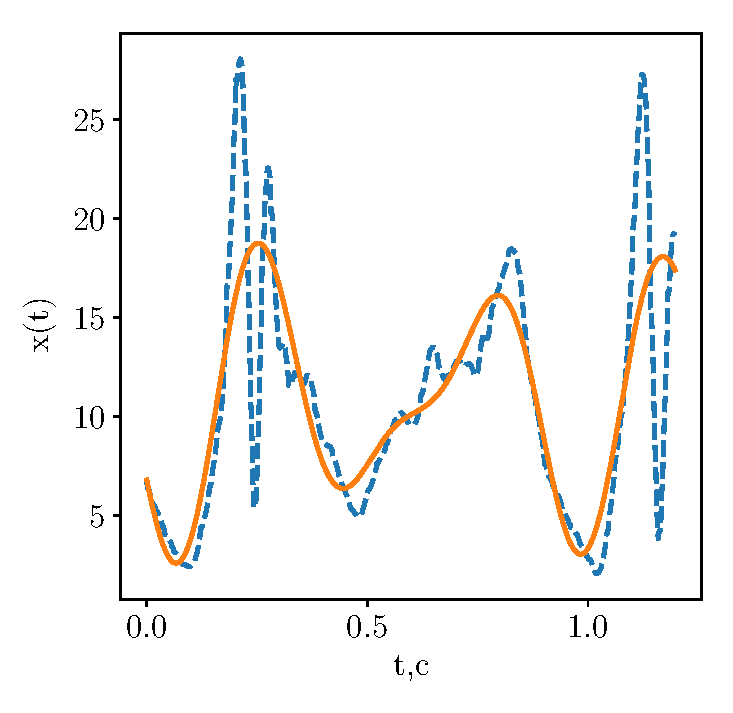
\includegraphics[width=0.3\textwidth]{figs/tr_init}}
  \subfloat[Фазовая траеткория (PCA)]{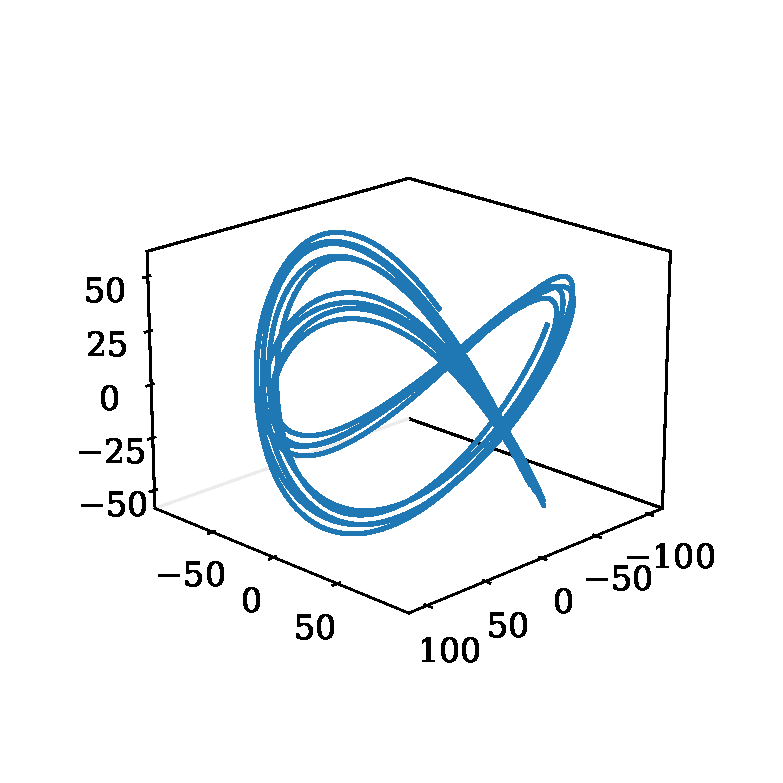
\includegraphics[width=0.3\textwidth]{figs/phase_init}}\\
\caption{Исследуемый временной ряд и его фазовая траетория. }
\label{fg:initial_traj}
\end{figure}

На рис.~\ref{fg:initial_traj} показан изначальный временной ряд и его разложение, пунктирной и сплошной линией соответственно, а также его фазовая траектория уменьшенная в пространство размерности 3 с помощью метода главных компонент (principal component analysis, PCA).

\section{Постановка задачи}
По имеющемуся временному ряду $\mathbf{s}=[s_1,...,s_N]^{\mathsf{T}}$ строится траекторная матрица или матрица Ганкеля

\begin{equation}
\mathbf{H_{s}} = 
\begin{bmatrix} 
	s_{1} & s_{2} & \ldots &s_{n-1} &s_{n}\\
	s_{2} & s_{3} & \ldots &s_{n} &s_{n+1}\\
	\vdots& \vdots & \ddots & \vdots & \vdots\\
	s_{N-n+1} & s_{N-n+2} &\ldots&s_{N-1} &s_{N}\\
\end{bmatrix}
\label{eq:hankel_matrix}
\end{equation}
                   
где $N$-длинна временного ряда, $n$-ширина окна, не меньшая, чем предполагаемый период. Обозначим $t$-ую строку матрицы Ганкеля $\mathbf{H_{s}}$ за $\mathbf{x_{t}}$. Матрица $\mathbf{H_{s}}$ пребразуется к:	
\begin{equation}
	\mathbf{H_{s}} = 
	\begin{bmatrix} 
                  	\mathbf{x_{1}}\\ \mathbf{x_{2}}\\
                  	\vdots\\
                  	\mathbf{x_{m}}\\
                   \end{bmatrix},
                   \mathbf{x_t}=[s_{t},s_{t+1},\ldots,s_{t+n-1}] ,
                   m = N-n+1
\label{eq:hankel_matrix_2}
\end{equation}
\vspace{\baselineskip}

Все векторы $\mathbf{x_{t}}$ принадлежат $\mathbb{H}_{\mathbf{x}} \subseteq \mathbb{R}^{n}$. Предполагается, что размерность траекторного пространства избыточна, поэтому предлагается исследовать некоторые проекции на траекторное подпространство.
Однако заранее неизвестно, в каком пространстве необходимо уменьшать размерность, поэтому задача приобретает следующий состоящий из двух вариантов вид:

\begin{equation}
	t \mapsto \mathbf{x} \mapsto \mathbb{H}_{x}^{n} \xrightarrow{} \mathbb{H}_{x}^{p} \xrightarrow{} \mathbb{S}_z^{(p)} \hookrightarrow [0,2\pi] \xrightarrow{f} r
\label{eq:goal}
\end{equation}

\vspace{\baselineskip}

\begin{Def}
Параметрическая аппроксимирующая модель временного ряда  $\mathbf{x}$  - это такое отображение $g$, что:
\begin{equation}
	g: \mathbb{R}^{q} \times \mathbf{S} \xrightarrow{} \mathbf{S}
\label{eq:param_model}
\end{equation}
\end{Def}

Предполагается, что аппроксимирующая модель строится в пространстве меньшей размерности $(p-1)$, в котором выбранное отображение $h: \mathbf{H}_{x}^{n} \xrightarrow{} \mathbf{S}_x^{(p-1)} $, где $(p-1)\ll n$, сохраняет геометрическую структуру множество точек $\mathbf{H}_{x}^{n}$. 

\begin{Def}
Структурная сложность - это количество параметров $q$ модели, позволяющих строить адекватную аппроксимацию.
\end{Def}



\section{Модели аппроксимации}
\paragraph{GAN для фазовых траекторий в 2D}

\begin{itemize}
\item \textbf{Модель генератор реальных данных}
\begin{equation}
	t \xrightarrow{} s\xrightarrow{Hankel}  \mathbf{x}_i \xrightarrow{PCA} x_i,
	\label{eq:GAN_real}
\end{equation}
где $x_i$ - точка фазовой траектории в уменьшенном пространстве, $x_i \in \mathbb{R}^2$.
\end{itemize}

\begin{itemize}
\item \textbf{Модель генератор синтетических данных}

\begin{equation}
	f_{ph}(\mathbf{w},\phi) = \sum_{j=0}^{l} w_{0,j}cos(j\phi) + i w_{1,j}sin(j\phi),
\label{eq:f_ph}
\end{equation}

\begin{equation}
	\phi \xrightarrow{f_{ph}} \hat{x}_{\phi},
	\quad
	\hat{x}_{\phi} = [real(f_{ph}),\:imag(f_{ph})],
	\quad
	\hat{x}_{\phi}  \in \mathbb{R}^2,
\label{eq:GAN_fake_1}
\end{equation}
\vspace{\baselineskip}

где $\mathbf{w}$ - вектор параметров (коэффициентов) тригонометрического ряда, $l$-количество пар коэффициентов.

Восстановление изначального временного ряда с помощью $f_{ph}$ можно представить в виде
\begin{equation}
	\phi \xrightarrow{f_{ph}} \hat{x}_{\phi} \xrightarrow{inverse~PCA}  \mathbf{x}_i \xrightarrow{inverse~Hankel}s
\label{eq:GAN_fake_2}
\end{equation}
\end{itemize}

\begin{itemize}
\item \textbf{Дискриминатор или функция потери и оптимизация}

Функцию потерь представляется в виде
\begin{equation}
\textrm{Loss}\mathbf{(\hat{x}_{\phi},x)} =  \sum_{i=1}^{101}\sum_{j=1}^{k}(\hat{x}_{\phi,i} - x_{i,j})^2
\label{eq:L}
\end{equation}
где для любого фиксированного $i$\; $\{x_{i,j}\}_1^k$ -- $k$ ближайших соседей к $\hat{x}_{\phi,i}$.

Решается задача оптимизации:
\begin{equation}
\mathbf{\hat{w}} = \argmin_{\mathbf{w} \in \mathbb{R}^{2l}} \textrm{Loss}(\mathbf{w}|\{x\})
\label{eq:arg_l}
\end{equation}
\end{itemize}

\paragraph{GAN для фазовых траекторий в 3D}

Предполагается, что структура модели проще в сферических координатах.
Построим отображение $x_p \in \mathbb{H}_{x}^{p} $ в $\mathbb{S}_{z}^{p-1} $ при $p = 2$.

\begin{equation}
	\phi: \mathbf{x}_p(t)  \xrightarrow{} \mathbf{z}_{(p-1)}(t) = [\alpha_{1} (t),..., \alpha_{p-1}(t), r{t}]
\label{eq:param_model2}
\end{equation}

В качестве базисных функций на поверхности 3 мерной сферы выберем сферические гармоники:

\begin{equation}
	Y_l^m(\alpha_1,\alpha_2) = \sqrt{ \frac{(2l+1)}{4\pi} \frac{(l-m)!}{(l+m)!} } P_l^m(cos\theta)e^{im\phi}
\label{eq:Yml}
\end{equation}

\begin{itemize}
\item \textbf{Модель генератор синтетических данных}

\begin{equation}
	f_{ph}(\mathbf{w},\alpha_1,\alpha_2) = \sum_{n,m \in N,M} w_{n,m}Y_l^m(\alpha_1,\alpha_2)
\label{eq:f_ph_3d}
\end{equation}
\vspace{\baselineskip}

\item \textbf{Дискриминатор или функция потери и оптимизация}

Функцию потерь представляется в виде
\begin{equation}
\textrm{Loss} =  \sum_{n,m \in N,M} \hat{f}_{ph}(\mathbf{w},\alpha_1,\alpha_2) - f_{real}(\alpha_{1},\alpha_2)
\label{eq:L_3d}
\end{equation}

Решается задача оптимизации:
\begin{equation}
\mathbf{\hat{w}} = \argmin_{\mathbf{w} \in \mathbb{R}^{2l}} \textrm{Loss}(\mathbf{w}|\{z_{2}\})
\label{eq:arg_l}
\end{equation}
\end{itemize}


\section{Эксперимент}

\paragraph{Аппроксимация сферическими гармониками 3D}

\begin{figure}[h]
\centering
\includegraphics[width=0.5\textwidth]{figs/3D_sp_harm}
\caption{Аппроксимация сферическими гармониками 3D. }
\label{fg:3D_sp_harm}
\end{figure}

\section{Заключение}
\newpage
\bibliographystyle{unsrt}
\bibliography{lib}

\end{document}
